
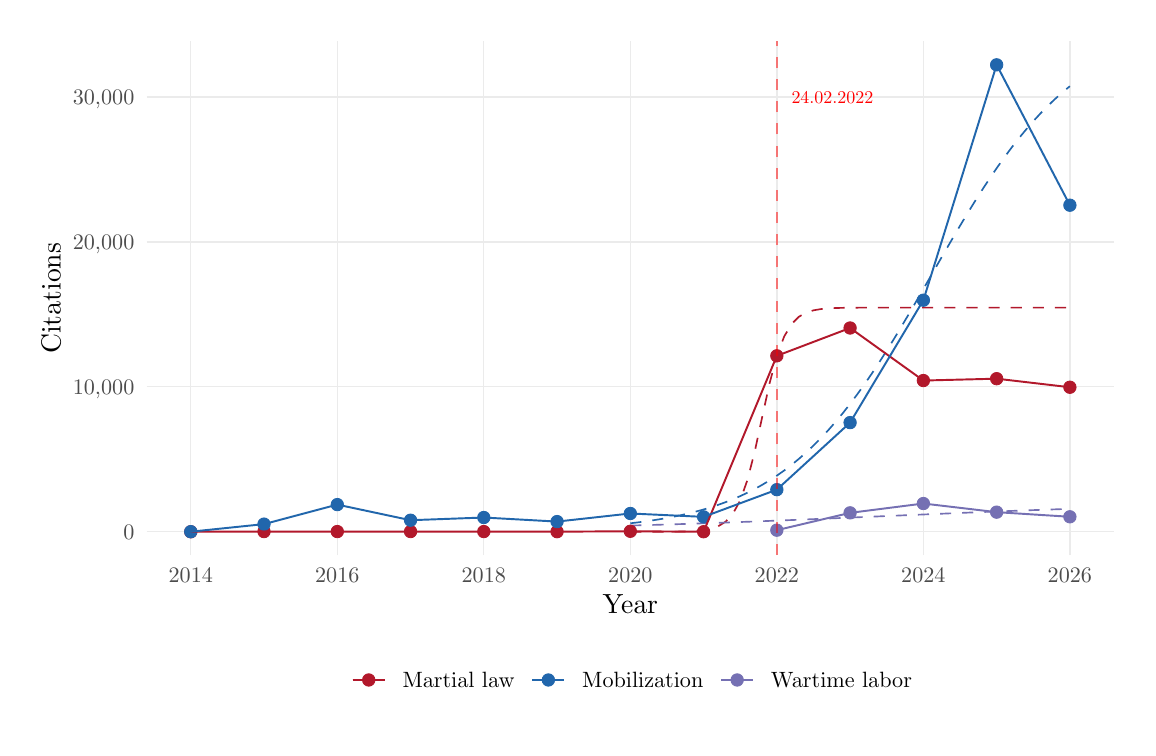
\begin{tikzpicture}[x=1pt,y=1pt]
\definecolor{fillColor}{RGB}{255,255,255}
\path[use as bounding box,fill=fillColor,fill opacity=0.00] (0,0) rectangle (397.48,252.94);
\begin{scope}
\path[clip] (  0.00,  0.00) rectangle (397.48,252.94);
\definecolor{fillColor}{RGB}{255,255,255}

\path[fill=fillColor] ( -0.00,  0.00) rectangle (397.48,252.94);
\end{scope}
\begin{scope}
\path[clip] ( 43.05, 62.35) rectangle (392.48,247.95);
\definecolor{drawColor}{gray}{0.92}

\path[draw=drawColor,line width= 0.5pt,line join=round] ( 43.05, 70.78) --
	(392.48, 70.78);

\path[draw=drawColor,line width= 0.5pt,line join=round] ( 43.05,123.17) --
	(392.48,123.17);

\path[draw=drawColor,line width= 0.5pt,line join=round] ( 43.05,175.55) --
	(392.48,175.55);

\path[draw=drawColor,line width= 0.5pt,line join=round] ( 43.05,227.94) --
	(392.48,227.94);

\path[draw=drawColor,line width= 0.5pt,line join=round] ( 58.93, 62.35) --
	( 58.93,247.95);

\path[draw=drawColor,line width= 0.5pt,line join=round] (111.88, 62.35) --
	(111.88,247.95);

\path[draw=drawColor,line width= 0.5pt,line join=round] (164.82, 62.35) --
	(164.82,247.95);

\path[draw=drawColor,line width= 0.5pt,line join=round] (217.77, 62.35) --
	(217.77,247.95);

\path[draw=drawColor,line width= 0.5pt,line join=round] (270.71, 62.35) --
	(270.71,247.95);

\path[draw=drawColor,line width= 0.5pt,line join=round] (323.66, 62.35) --
	(323.66,247.95);

\path[draw=drawColor,line width= 0.5pt,line join=round] (376.60, 62.35) --
	(376.60,247.95);
\definecolor{drawColor}{RGB}{178,24,43}

\path[draw=drawColor,line width= 0.6pt,dash pattern=on 4pt off 4pt ,line join=round] (217.77, 70.79) --
	(220.41, 70.79) --
	(223.06, 70.79) --
	(225.71, 70.79) --
	(228.36, 70.80) --
	(231.00, 70.81) --
	(233.65, 70.83) --
	(236.30, 70.87) --
	(238.94, 70.95) --
	(241.59, 71.10) --
	(244.24, 71.37) --
	(246.89, 71.87) --
	(249.53, 72.78) --
	(252.18, 74.42) --
	(254.83, 77.30) --
	(257.48, 82.12) --
	(260.12, 89.62) --
	(262.77, 99.99) --
	(265.42,112.26) --
	(268.06,124.35) --
	(270.71,134.31) --
	(273.36,141.35) --
	(276.01,145.82) --
	(278.65,148.47) --
	(281.30,149.97) --
	(283.95,150.80) --
	(286.60,151.25) --
	(289.24,151.50) --
	(291.89,151.63) --
	(294.54,151.70) --
	(297.18,151.74) --
	(299.83,151.76) --
	(302.48,151.77) --
	(305.13,151.78) --
	(307.77,151.78) --
	(310.42,151.78) --
	(313.07,151.78) --
	(315.71,151.78) --
	(318.36,151.78) --
	(321.01,151.78) --
	(323.66,151.78) --
	(326.30,151.78) --
	(328.95,151.78) --
	(331.60,151.78) --
	(334.25,151.78) --
	(336.89,151.78) --
	(339.54,151.78) --
	(342.19,151.78) --
	(344.83,151.78) --
	(347.48,151.78) --
	(350.13,151.78) --
	(352.78,151.78) --
	(355.42,151.78) --
	(358.07,151.78) --
	(360.72,151.78) --
	(363.37,151.78) --
	(366.01,151.78) --
	(368.66,151.78) --
	(371.31,151.78) --
	(373.95,151.78) --
	(376.60,151.78);
\definecolor{drawColor}{RGB}{33,102,172}

\path[draw=drawColor,line width= 0.6pt,dash pattern=on 4pt off 4pt ,line join=round] (217.77, 73.85) --
	(220.41, 74.16) --
	(223.06, 74.51) --
	(225.71, 74.89) --
	(228.36, 75.31) --
	(231.00, 75.77) --
	(233.65, 76.27) --
	(236.30, 76.83) --
	(238.94, 77.44) --
	(241.59, 78.11) --
	(244.24, 78.84) --
	(246.89, 79.64) --
	(249.53, 80.52) --
	(252.18, 81.48) --
	(254.83, 82.53) --
	(257.48, 83.67) --
	(260.12, 84.91) --
	(262.77, 86.27) --
	(265.42, 87.74) --
	(268.06, 89.34) --
	(270.71, 91.06) --
	(273.36, 92.93) --
	(276.01, 94.94) --
	(278.65, 97.11) --
	(281.30, 99.44) --
	(283.95,101.93) --
	(286.60,104.60) --
	(289.24,107.43) --
	(291.89,110.45) --
	(294.54,113.63) --
	(297.18,117.00) --
	(299.83,120.53) --
	(302.48,124.24) --
	(305.13,128.10) --
	(307.77,132.11) --
	(310.42,136.26) --
	(313.07,140.53) --
	(315.71,144.91) --
	(318.36,149.38) --
	(321.01,153.92) --
	(323.66,158.50) --
	(326.30,163.11) --
	(328.95,167.72) --
	(331.60,172.31) --
	(334.25,176.86) --
	(336.89,181.34) --
	(339.54,185.74) --
	(342.19,190.04) --
	(344.83,194.21) --
	(347.48,198.25) --
	(350.13,202.15) --
	(352.78,205.88) --
	(355.42,209.45) --
	(358.07,212.85) --
	(360.72,216.08) --
	(363.37,219.13) --
	(366.01,222.00) --
	(368.66,224.70) --
	(371.31,227.23) --
	(373.95,229.59) --
	(376.60,231.79);
\definecolor{drawColor}{RGB}{117,112,179}

\path[draw=drawColor,line width= 0.6pt,dash pattern=on 4pt off 4pt ,line join=round] (217.77, 73.02) --
	(220.41, 73.10) --
	(223.06, 73.17) --
	(225.71, 73.25) --
	(228.36, 73.33) --
	(231.00, 73.41) --
	(233.65, 73.49) --
	(236.30, 73.57) --
	(238.94, 73.66) --
	(241.59, 73.75) --
	(244.24, 73.84) --
	(246.89, 73.93) --
	(249.53, 74.02) --
	(252.18, 74.11) --
	(254.83, 74.21) --
	(257.48, 74.31) --
	(260.12, 74.40) --
	(262.77, 74.50) --
	(265.42, 74.60) --
	(268.06, 74.71) --
	(270.71, 74.81) --
	(273.36, 74.92) --
	(276.01, 75.02) --
	(278.65, 75.13) --
	(281.30, 75.24) --
	(283.95, 75.35) --
	(286.60, 75.46) --
	(289.24, 75.57) --
	(291.89, 75.68) --
	(294.54, 75.79) --
	(297.18, 75.90) --
	(299.83, 76.01) --
	(302.48, 76.13) --
	(305.13, 76.24) --
	(307.77, 76.35) --
	(310.42, 76.47) --
	(313.07, 76.58) --
	(315.71, 76.69) --
	(318.36, 76.81) --
	(321.01, 76.92) --
	(323.66, 77.03) --
	(326.30, 77.14) --
	(328.95, 77.25) --
	(331.60, 77.36) --
	(334.25, 77.47) --
	(336.89, 77.58) --
	(339.54, 77.69) --
	(342.19, 77.80) --
	(344.83, 77.90) --
	(347.48, 78.01) --
	(350.13, 78.11) --
	(352.78, 78.21) --
	(355.42, 78.31) --
	(358.07, 78.41) --
	(360.72, 78.51) --
	(363.37, 78.61) --
	(366.01, 78.70) --
	(368.66, 78.80) --
	(371.31, 78.89) --
	(373.95, 78.98) --
	(376.60, 79.07);
\definecolor{drawColor}{RGB}{178,24,43}
\definecolor{fillColor}{RGB}{178,24,43}

\path[draw=drawColor,line width= 0.3pt,line join=round,line cap=round,fill=fillColor] ( 58.93, 70.79) circle (  2.25);

\path[draw=drawColor,line width= 0.3pt,line join=round,line cap=round,fill=fillColor] ( 85.40, 70.85) circle (  2.25);

\path[draw=drawColor,line width= 0.3pt,line join=round,line cap=round,fill=fillColor] (111.88, 70.86) circle (  2.25);

\path[draw=drawColor,line width= 0.3pt,line join=round,line cap=round,fill=fillColor] (138.35, 70.86) circle (  2.25);

\path[draw=drawColor,line width= 0.3pt,line join=round,line cap=round,fill=fillColor] (164.82, 70.86) circle (  2.25);

\path[draw=drawColor,line width= 0.3pt,line join=round,line cap=round,fill=fillColor] (191.29, 70.82) circle (  2.25);

\path[draw=drawColor,line width= 0.3pt,line join=round,line cap=round,fill=fillColor] (217.77, 70.96) circle (  2.25);

\path[draw=drawColor,line width= 0.3pt,line join=round,line cap=round,fill=fillColor] (244.24, 70.80) circle (  2.25);

\path[draw=drawColor,line width= 0.3pt,line join=round,line cap=round,fill=fillColor] (270.71,134.36) circle (  2.25);

\path[draw=drawColor,line width= 0.3pt,line join=round,line cap=round,fill=fillColor] (297.18,144.42) circle (  2.25);

\path[draw=drawColor,line width= 0.3pt,line join=round,line cap=round,fill=fillColor] (323.66,125.43) circle (  2.25);

\path[draw=drawColor,line width= 0.3pt,line join=round,line cap=round,fill=fillColor] (350.13,126.10) circle (  2.25);

\path[draw=drawColor,line width= 0.3pt,line join=round,line cap=round,fill=fillColor] (376.60,123.01) circle (  2.25);
\definecolor{drawColor}{RGB}{33,102,172}
\definecolor{fillColor}{RGB}{33,102,172}

\path[draw=drawColor,line width= 0.3pt,line join=round,line cap=round,fill=fillColor] ( 58.93, 70.81) circle (  2.25);

\path[draw=drawColor,line width= 0.3pt,line join=round,line cap=round,fill=fillColor] ( 85.40, 73.55) circle (  2.25);

\path[draw=drawColor,line width= 0.3pt,line join=round,line cap=round,fill=fillColor] (111.88, 80.60) circle (  2.25);

\path[draw=drawColor,line width= 0.3pt,line join=round,line cap=round,fill=fillColor] (138.35, 74.96) circle (  2.25);

\path[draw=drawColor,line width= 0.3pt,line join=round,line cap=round,fill=fillColor] (164.82, 75.93) circle (  2.25);

\path[draw=drawColor,line width= 0.3pt,line join=round,line cap=round,fill=fillColor] (191.29, 74.46) circle (  2.25);

\path[draw=drawColor,line width= 0.3pt,line join=round,line cap=round,fill=fillColor] (217.77, 77.39) circle (  2.25);

\path[draw=drawColor,line width= 0.3pt,line join=round,line cap=round,fill=fillColor] (244.24, 76.17) circle (  2.25);

\path[draw=drawColor,line width= 0.3pt,line join=round,line cap=round,fill=fillColor] (270.71, 86.00) circle (  2.25);

\path[draw=drawColor,line width= 0.3pt,line join=round,line cap=round,fill=fillColor] (297.18,110.23) circle (  2.25);

\path[draw=drawColor,line width= 0.3pt,line join=round,line cap=round,fill=fillColor] (323.66,154.46) circle (  2.25);

\path[draw=drawColor,line width= 0.3pt,line join=round,line cap=round,fill=fillColor] (350.13,239.51) circle (  2.25);

\path[draw=drawColor,line width= 0.3pt,line join=round,line cap=round,fill=fillColor] (376.60,188.79) circle (  2.25);
\definecolor{drawColor}{RGB}{117,112,179}
\definecolor{fillColor}{RGB}{117,112,179}

\path[draw=drawColor,line width= 0.3pt,line join=round,line cap=round,fill=fillColor] (270.71, 71.36) circle (  2.25);

\path[draw=drawColor,line width= 0.3pt,line join=round,line cap=round,fill=fillColor] (297.18, 77.62) circle (  2.25);

\path[draw=drawColor,line width= 0.3pt,line join=round,line cap=round,fill=fillColor] (323.66, 80.99) circle (  2.25);

\path[draw=drawColor,line width= 0.3pt,line join=round,line cap=round,fill=fillColor] (350.13, 77.87) circle (  2.25);

\path[draw=drawColor,line width= 0.3pt,line join=round,line cap=round,fill=fillColor] (376.60, 76.20) circle (  2.25);
\definecolor{drawColor}{RGB}{178,24,43}

\path[draw=drawColor,line width= 0.7pt,line join=round] ( 58.93, 70.79) --
	( 85.40, 70.85) --
	(111.88, 70.86) --
	(138.35, 70.86) --
	(164.82, 70.86) --
	(191.29, 70.82) --
	(217.77, 70.96) --
	(244.24, 70.80) --
	(270.71,134.36) --
	(297.18,144.42) --
	(323.66,125.43) --
	(350.13,126.10) --
	(376.60,123.01);
\definecolor{drawColor}{RGB}{33,102,172}

\path[draw=drawColor,line width= 0.7pt,line join=round] ( 58.93, 70.81) --
	( 85.40, 73.55) --
	(111.88, 80.60) --
	(138.35, 74.96) --
	(164.82, 75.93) --
	(191.29, 74.46) --
	(217.77, 77.39) --
	(244.24, 76.17) --
	(270.71, 86.00) --
	(297.18,110.23) --
	(323.66,154.46) --
	(350.13,239.51) --
	(376.60,188.79);
\definecolor{drawColor}{RGB}{117,112,179}

\path[draw=drawColor,line width= 0.7pt,line join=round] (270.71, 71.36) --
	(297.18, 77.62) --
	(323.66, 80.99) --
	(350.13, 77.87) --
	(376.60, 76.20);
\definecolor{drawColor}{RGB}{255,0,0}

\path[draw=drawColor,draw opacity=0.50,line width= 0.5pt,dash pattern=on 4pt off 4pt ,line join=round] (270.71, 62.35) -- (270.71,247.95);
\definecolor{drawColor}{RGB}{255,0,0}

\node[text=drawColor,anchor=base west,inner sep=0pt, outer sep=0pt, scale=  0.65] at (276.01,225.68) {24.02.2022};
\end{scope}
\begin{scope}
\path[clip] (  0.00,  0.00) rectangle (397.48,252.94);
\definecolor{drawColor}{gray}{0.30}

\node[text=drawColor,anchor=base east,inner sep=0pt, outer sep=0pt, scale=  0.80] at ( 38.55, 68.03) {0};

\node[text=drawColor,anchor=base east,inner sep=0pt, outer sep=0pt, scale=  0.80] at ( 38.55,120.41) {10,000};

\node[text=drawColor,anchor=base east,inner sep=0pt, outer sep=0pt, scale=  0.80] at ( 38.55,172.80) {20,000};

\node[text=drawColor,anchor=base east,inner sep=0pt, outer sep=0pt, scale=  0.80] at ( 38.55,225.18) {30,000};
\end{scope}
\begin{scope}
\path[clip] (  0.00,  0.00) rectangle (397.48,252.94);
\definecolor{drawColor}{gray}{0.30}

\node[text=drawColor,anchor=base,inner sep=0pt, outer sep=0pt, scale=  0.80] at ( 58.93, 52.34) {2014};

\node[text=drawColor,anchor=base,inner sep=0pt, outer sep=0pt, scale=  0.80] at (111.88, 52.34) {2016};

\node[text=drawColor,anchor=base,inner sep=0pt, outer sep=0pt, scale=  0.80] at (164.82, 52.34) {2018};

\node[text=drawColor,anchor=base,inner sep=0pt, outer sep=0pt, scale=  0.80] at (217.77, 52.34) {2020};

\node[text=drawColor,anchor=base,inner sep=0pt, outer sep=0pt, scale=  0.80] at (270.71, 52.34) {2022};

\node[text=drawColor,anchor=base,inner sep=0pt, outer sep=0pt, scale=  0.80] at (323.66, 52.34) {2024};

\node[text=drawColor,anchor=base,inner sep=0pt, outer sep=0pt, scale=  0.80] at (376.60, 52.34) {2026};
\end{scope}
\begin{scope}
\path[clip] (  0.00,  0.00) rectangle (397.48,252.94);
\definecolor{drawColor}{RGB}{0,0,0}

\node[text=drawColor,anchor=base,inner sep=0pt, outer sep=0pt, scale=  1.00] at (217.77, 41.40) {Year};
\end{scope}
\begin{scope}
\path[clip] (  0.00,  0.00) rectangle (397.48,252.94);
\definecolor{drawColor}{RGB}{0,0,0}

\node[text=drawColor,rotate= 90.00,anchor=base,inner sep=0pt, outer sep=0pt, scale=  1.00] at ( 11.89,155.15) {Citations};
\end{scope}
\begin{scope}
\path[clip] (  0.00,  0.00) rectangle (397.48,252.94);
\definecolor{drawColor}{RGB}{178,24,43}

\path[draw=drawColor,line width= 0.6pt,dash pattern=on 4pt off 4pt ,line join=round] (117.46, 17.23) -- (129.02, 17.23);
\definecolor{fillColor}{RGB}{178,24,43}

\path[draw=drawColor,line width= 0.3pt,line join=round,line cap=round,fill=fillColor] (123.24, 17.23) circle (  2.25);

\path[draw=drawColor,line width= 0.7pt,line join=round] (117.46, 17.23) -- (129.02, 17.23);
\end{scope}
\begin{scope}
\path[clip] (  0.00,  0.00) rectangle (397.48,252.94);
\definecolor{drawColor}{RGB}{33,102,172}

\path[draw=drawColor,line width= 0.6pt,dash pattern=on 4pt off 4pt ,line join=round] (182.37, 17.23) -- (193.93, 17.23);
\definecolor{fillColor}{RGB}{33,102,172}

\path[draw=drawColor,line width= 0.3pt,line join=round,line cap=round,fill=fillColor] (188.15, 17.23) circle (  2.25);

\path[draw=drawColor,line width= 0.7pt,line join=round] (182.37, 17.23) -- (193.93, 17.23);
\end{scope}
\begin{scope}
\path[clip] (  0.00,  0.00) rectangle (397.48,252.94);
\definecolor{drawColor}{RGB}{117,112,179}

\path[draw=drawColor,line width= 0.6pt,dash pattern=on 4pt off 4pt ,line join=round] (250.59, 17.23) -- (262.15, 17.23);
\definecolor{fillColor}{RGB}{117,112,179}

\path[draw=drawColor,line width= 0.3pt,line join=round,line cap=round,fill=fillColor] (256.37, 17.23) circle (  2.25);

\path[draw=drawColor,line width= 0.7pt,line join=round] (250.59, 17.23) -- (262.15, 17.23);
\end{scope}
\begin{scope}
\path[clip] (  0.00,  0.00) rectangle (397.48,252.94);
\definecolor{drawColor}{RGB}{0,0,0}

\node[text=drawColor,anchor=base west,inner sep=0pt, outer sep=0pt, scale=  0.80] at (135.47, 14.47) {Martial law};
\end{scope}
\begin{scope}
\path[clip] (  0.00,  0.00) rectangle (397.48,252.94);
\definecolor{drawColor}{RGB}{0,0,0}

\node[text=drawColor,anchor=base west,inner sep=0pt, outer sep=0pt, scale=  0.80] at (200.38, 14.47) {Mobilization};
\end{scope}
\begin{scope}
\path[clip] (  0.00,  0.00) rectangle (397.48,252.94);
\definecolor{drawColor}{RGB}{0,0,0}

\node[text=drawColor,anchor=base west,inner sep=0pt, outer sep=0pt, scale=  0.80] at (268.60, 14.47) {Wartime labor};
\end{scope}
\end{tikzpicture}

